\begin{appendix}

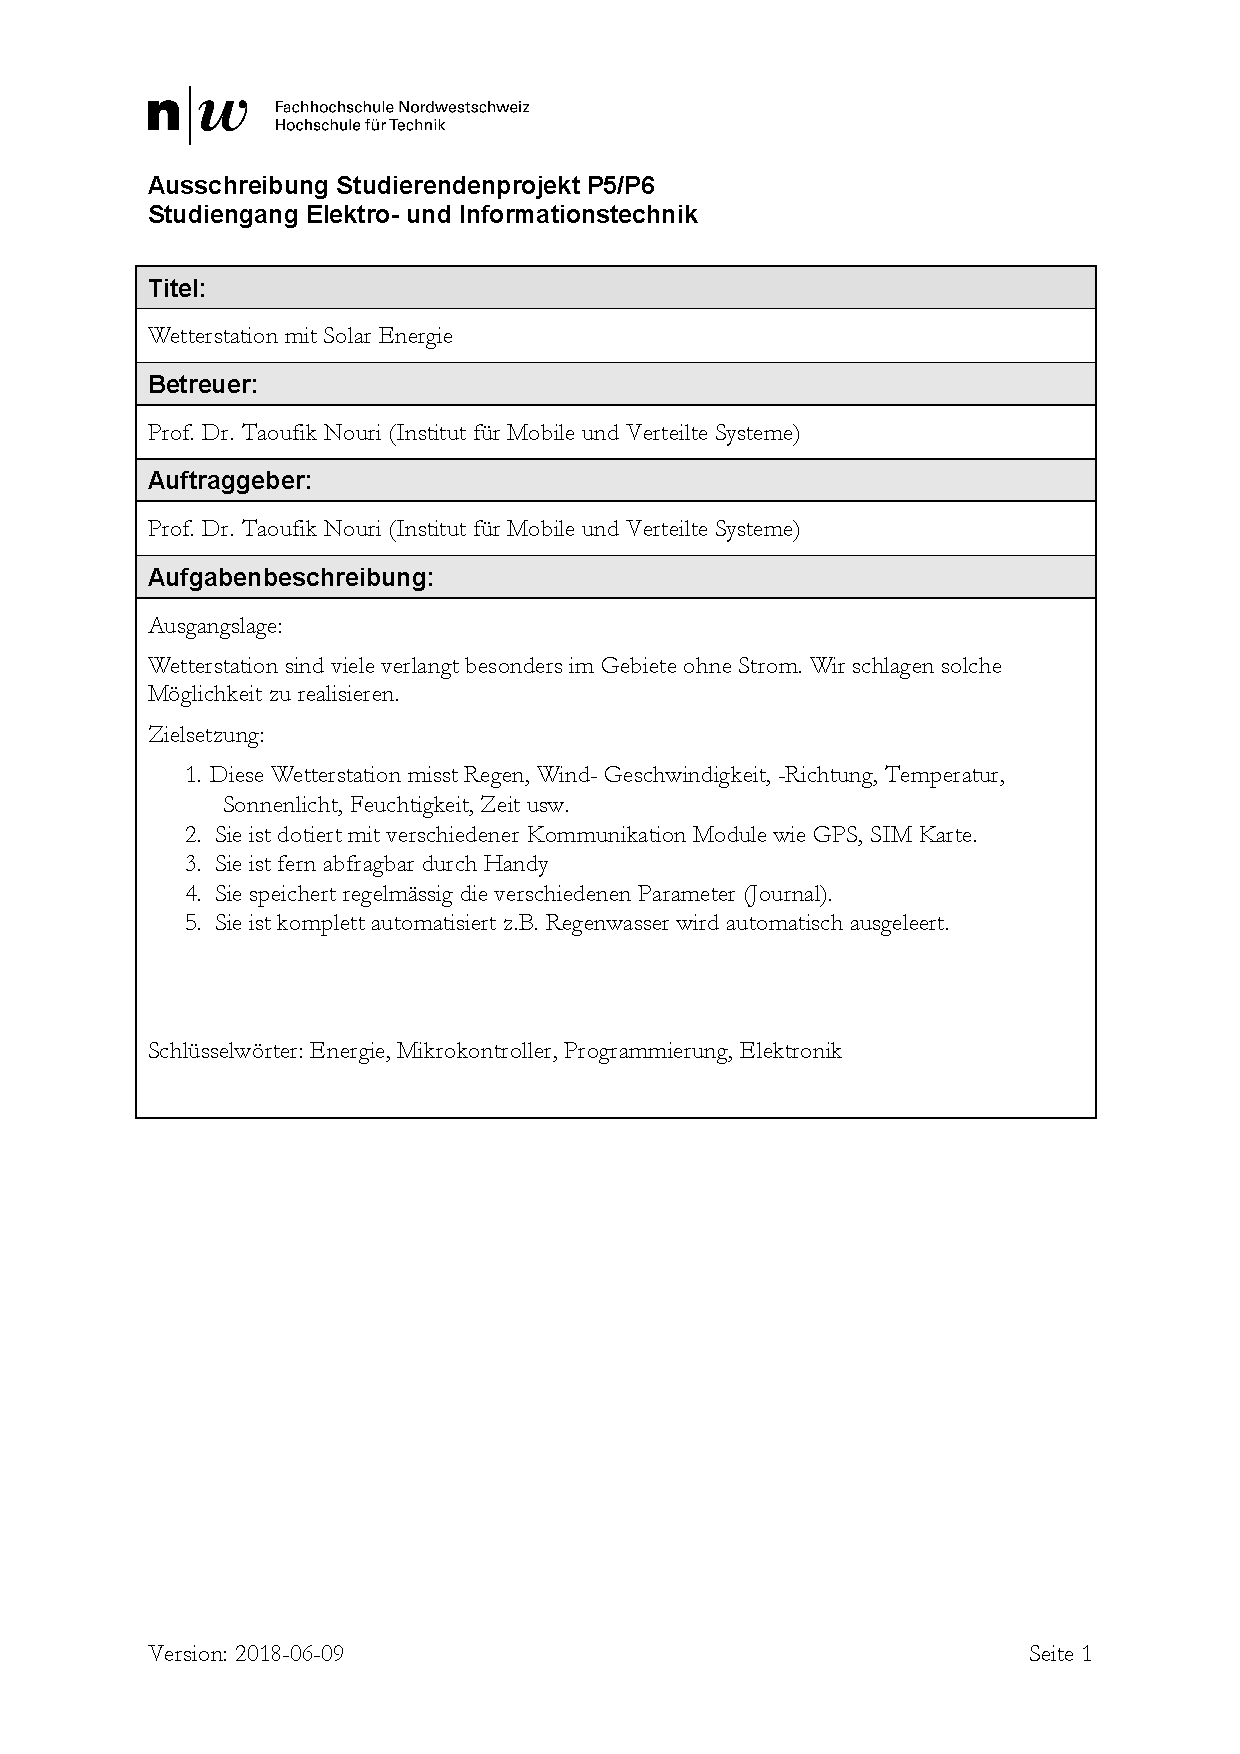
\includepdf[pages={1},nup=1x1,landscape=false,scale=0.85,offset=0 -40,pagecommand={\section{Lastenheft}\label{appendix:Lastenheft}}]{appendix/Auftragsbeschreibung.pdf} 

\newpage

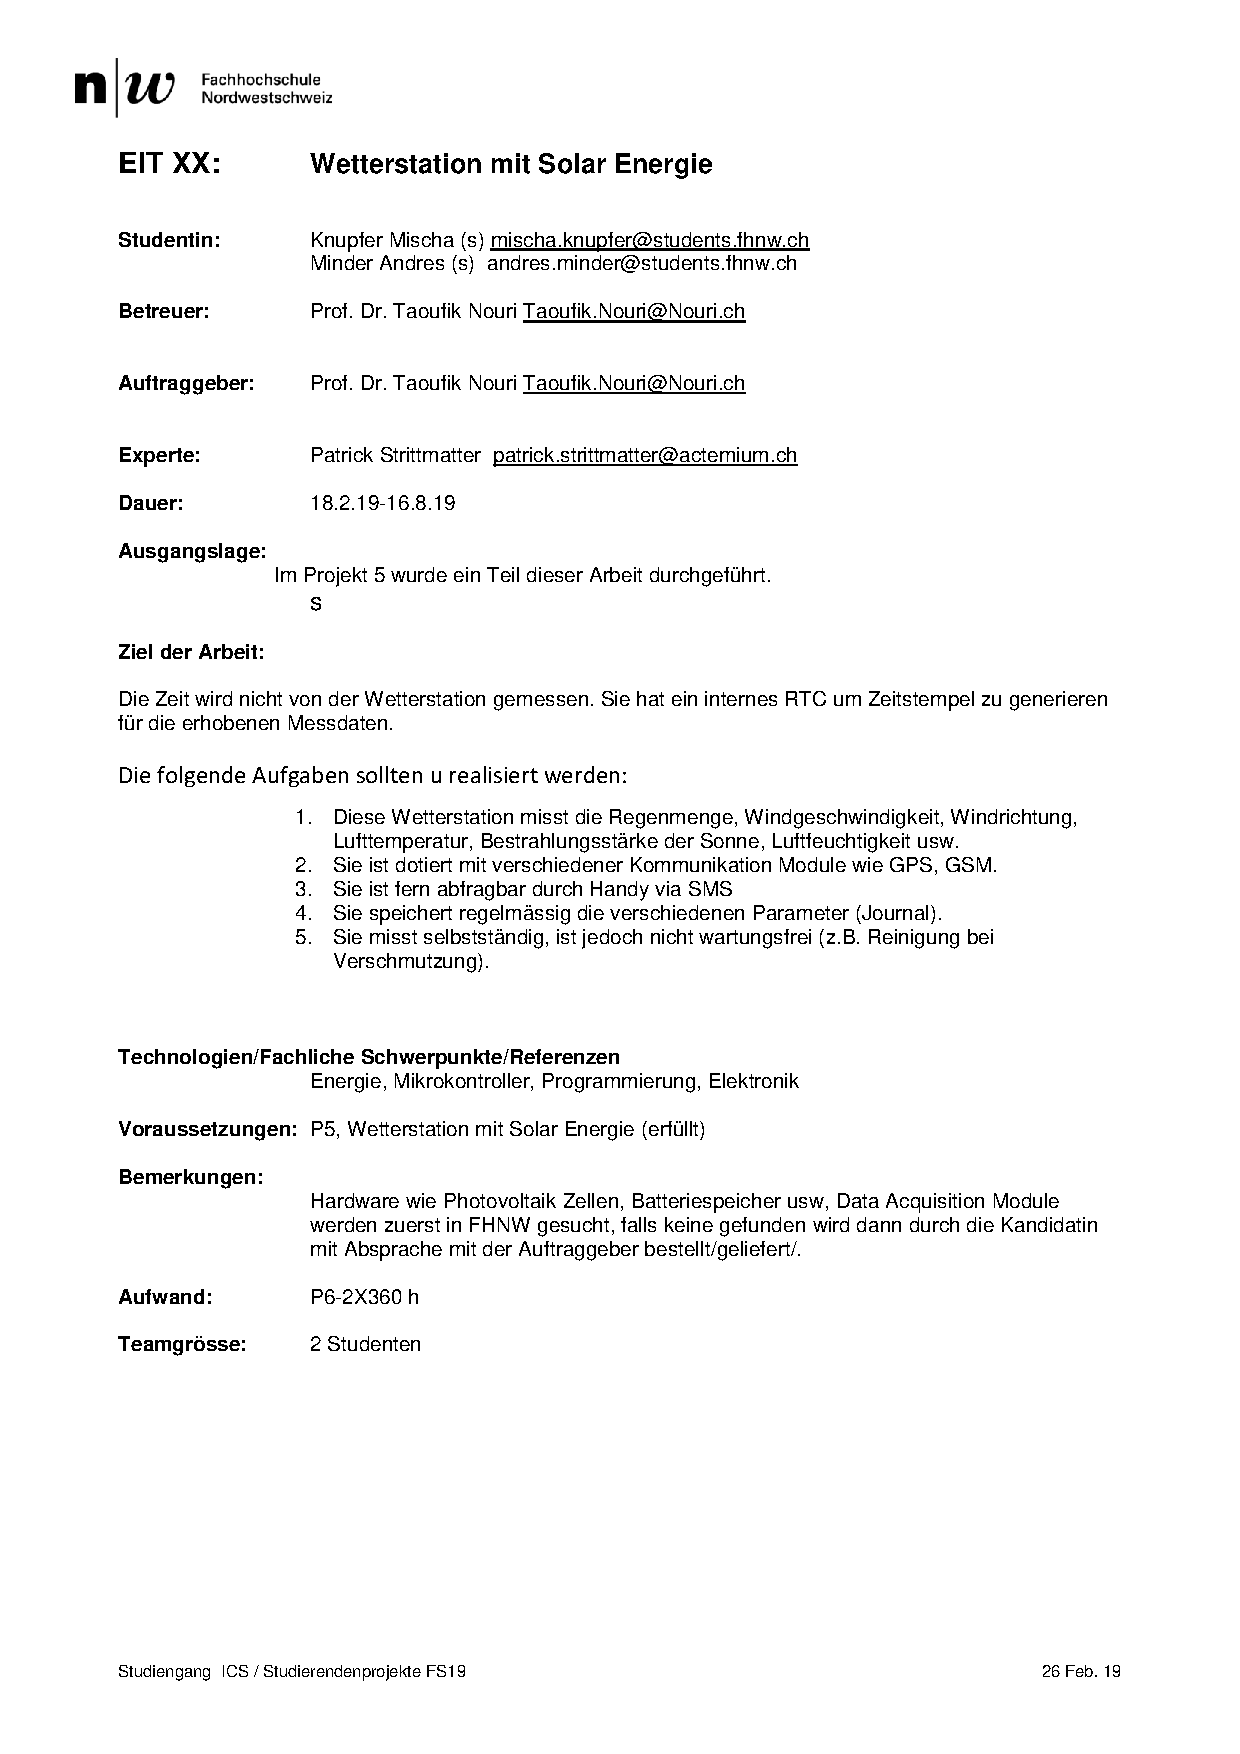
\includepdf[pages={1},nup=1x1,landscape=false,scale=0.85,offset=0 -40,pagecommand={\section{Aufgabenstellung}\label{appendix:aufgabenstellung}\thispagestyle{myheadings}}]{appendix/Aufgabenstellung.pdf} 

\newpage

\section{Lizenz-Texte}
\label{sec:lizenztexte}
\subsection{Adafruit\_BME280}
\label{subsec:adafruit_bme280_lizenztext}
Copyright (c) 2015, Limor Fried \& Kevin Townsend for Adafruit Industries 
All rights reserved.\\

Redistribution and use in source and binary forms, with or without 
modification, are permitted provided that the following conditions are met:
\begin{itemize}
	\item[*] Redistributions of source code must retain the above copyright notice, this list of conditions and the following disclaimer.
	\item[*] Redistributions in binary form must reproduce the above copyright notice, this list of conditions and the following disclaimer in the documentation and/or other materials provided with the distribution.
	\item[*] Neither the name of Adafruit Industries nor the names of its contributors may be used to endorse or promote products derived from this software without specific prior written permission.\\
\end{itemize}

THIS SOFTWARE IS PROVIDED BY THE COPYRIGHT HOLDERS AND CONTRIBUTORS \glqq AS IS\grqq AND ANY EXPRESS OR IMPLIED WARRANTIES, INCLUDING, BUT NOT LIMITED TO, THE IMPLIED WARRANTIES OF MERCHANTABILITY AND FITNESS FOR A PARTICULAR PURPOSE ARE DISCLAIMED. IN NO EVENT SHALL THE COPYRIGHT OWNER OR CONTRIBUTORS BE LIABLE FOR ANY DIRECT, INDIRECT, INCIDENTAL, SPECIAL, EXEMPLARY, OR CONSEQUENTIAL DAMAGES (INCLUDING, BUT NOT LIMITED TO, PROCUREMENT OF SUBSTITUTE GOODS OR SERVICES; LOSS OF USE, DATA, OR PROFITS; OR BUSINESS INTERRUPTION) HOWEVER CAUSED AND ON ANY THEORY OF LIABILITY, WHETHER IN CONTRACT, STRICT LIABILITY, OR TORT (INCLUDING NEGLIGENCE OR OTHERWISE) ARISING IN ANY WAY OUT OF THE USE OF THIS SOFTWARE, EVEN IF ADVISED OF THE POSSIBILITY OF SUCH DAMAGE. \cite{license_bme280}\\

\subsection{RTClib}
\label{subsec:rtclib_lizenztext}
MIT License\\

Copyright (c) 2019 Adafruit Industries\\

Permission is hereby granted, free of charge, to any person obtaining a copy of this software and associated documentation files (the \glqq Software\grqq), to deal in the Software without restriction, including without limitation the rights to use, copy, modify, merge, publish, distribute, sublicense, and/or sell copies of the Software, and to permit persons to whom the Software is furnished to do so, subject to the following conditions:\\

The above copyright notice and this permission notice shall be included in all copies or substantial portions of the Software.\\

THE SOFTWARE IS PROVIDED \glqq AS IS\grqq, WITHOUT WARRANTY OF ANY KIND, EXPRESS OR IMPLIED, INCLUDING BUT NOT LIMITED TO THE WARRANTIES OF MERCHANTABILITY, FITNESS FOR A PARTICULAR PURPOSE AND NONINFRINGEMENT. IN NO EVENT SHALL THE AUTHORS OR COPYRIGHT HOLDERS BE LIABLE FOR ANY CLAIM, DAMAGES OR OTHER LIABILITY, WHETHER IN AN ACTION OF CONTRACT, TORT OR OTHERWISE, ARISING FROM, OUT OF OR IN CONNECTION WITH THE SOFTWARE OR THE USE OR OTHER DEALINGS IN THE SOFTWARE. \cite{license_rtclib}\\

\newpage

\section{Konzept Posterbild}
\label{sec:konzept_posterbild}
\begin{figure}[h]
\centering
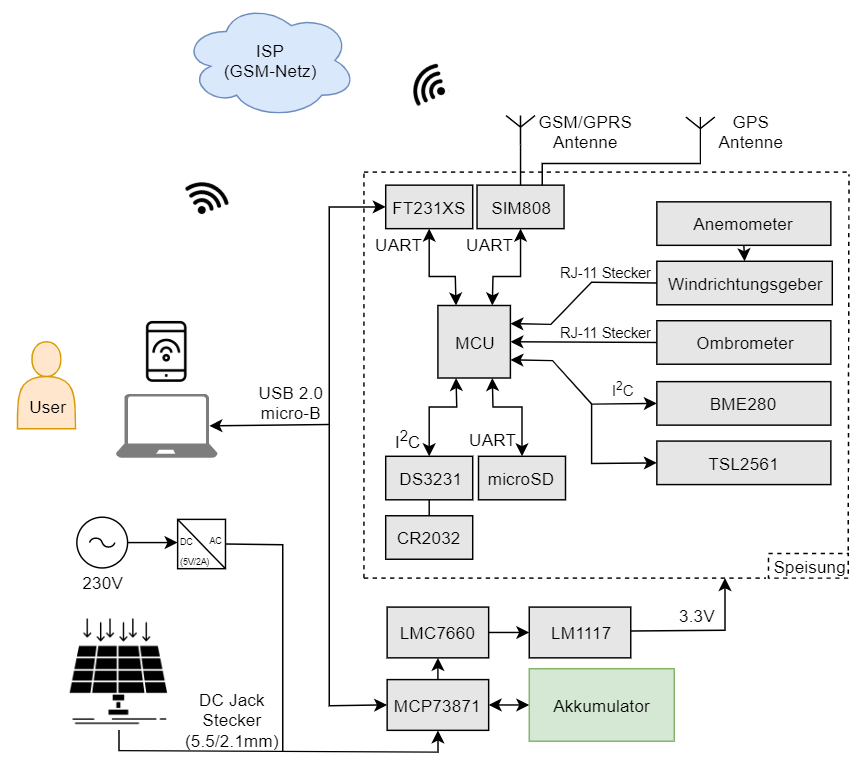
\includegraphics[width=\textwidth]{graphics/Konzeptdiagramme/komplett.PNG}
\caption{Komplette Darstellung des Konzepts}
\label{fig:konzept_posterbild}
\end{figure}
\newpage
\begin{landscape}
\section{Schema}
\label{Anhang:Schema}
\begin{figure}[h]
\centering
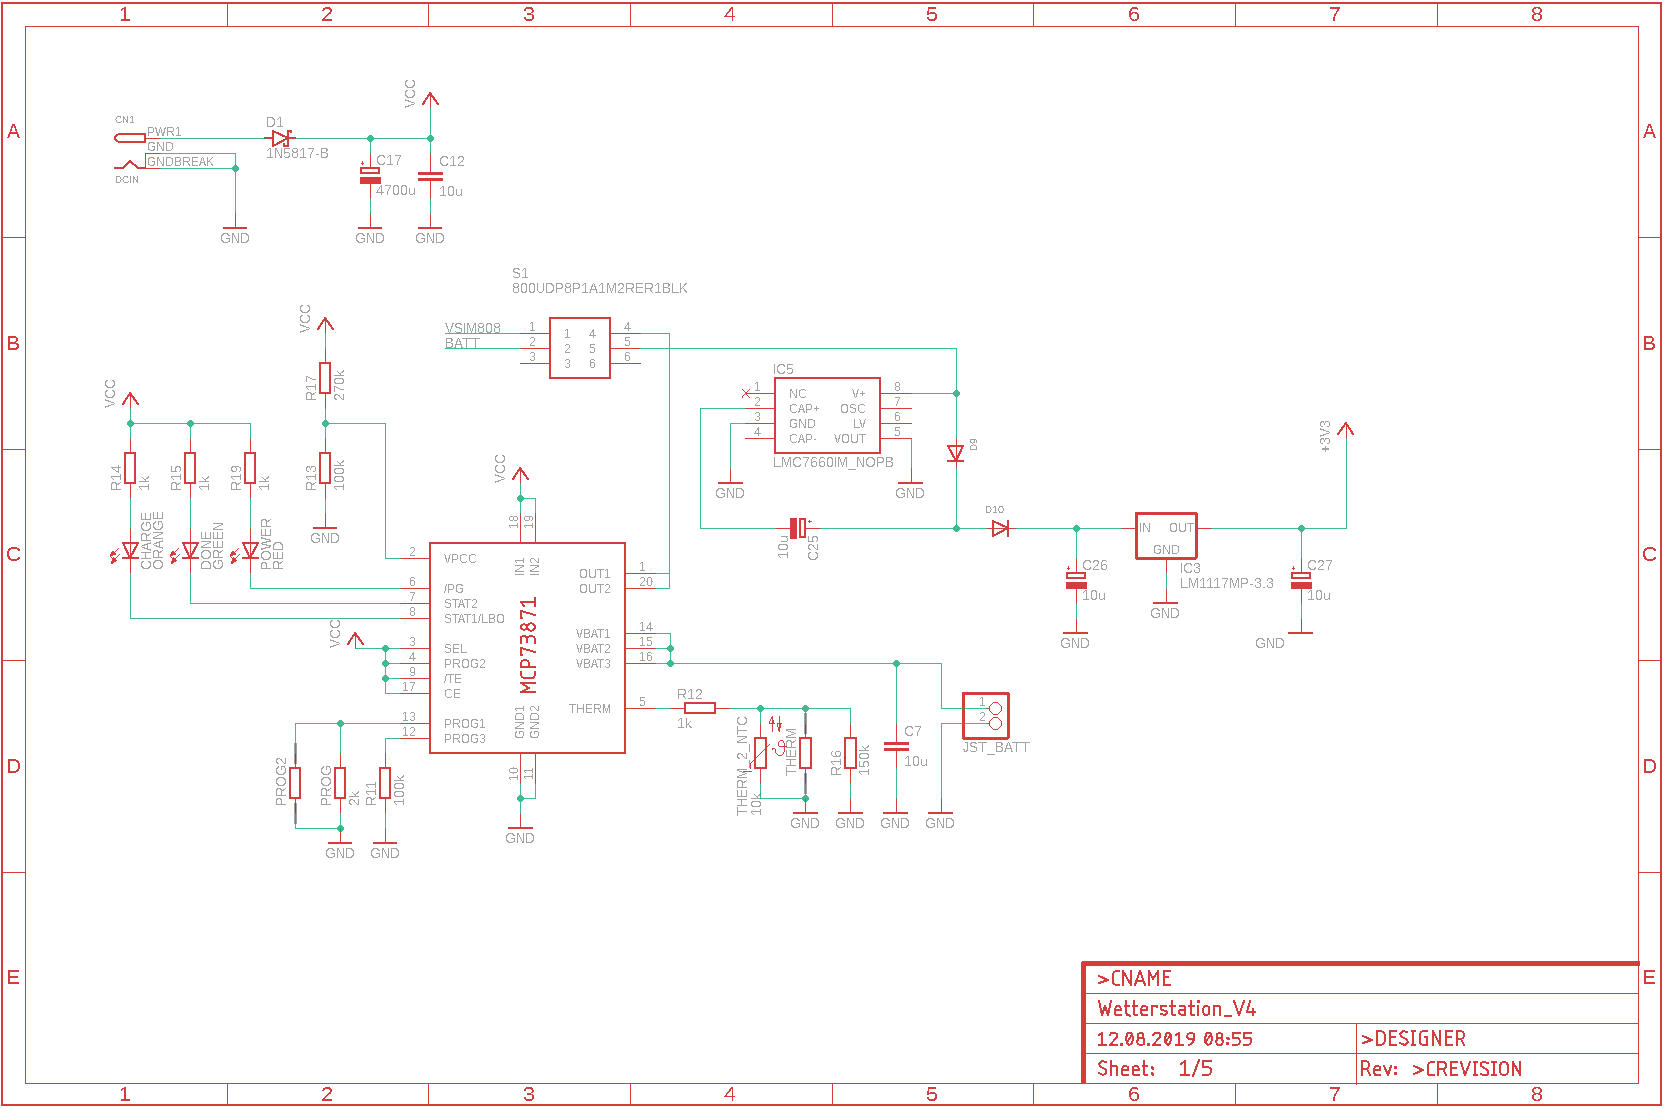
\includegraphics[width=0.66\linewidth]{graphics/Anhang_Eagle/PowerSupply.png}
\caption{Schema der Energieversorgung.}
\label{fig:Anhang_PowerSupply}
\end{figure}
Abbildung \ref{fig:Anhang_PowerSupply} zeigt das Schema der Energieversorgungs-Bauteilgruppe.
\newpage
\begin{figure}[h]
\centering
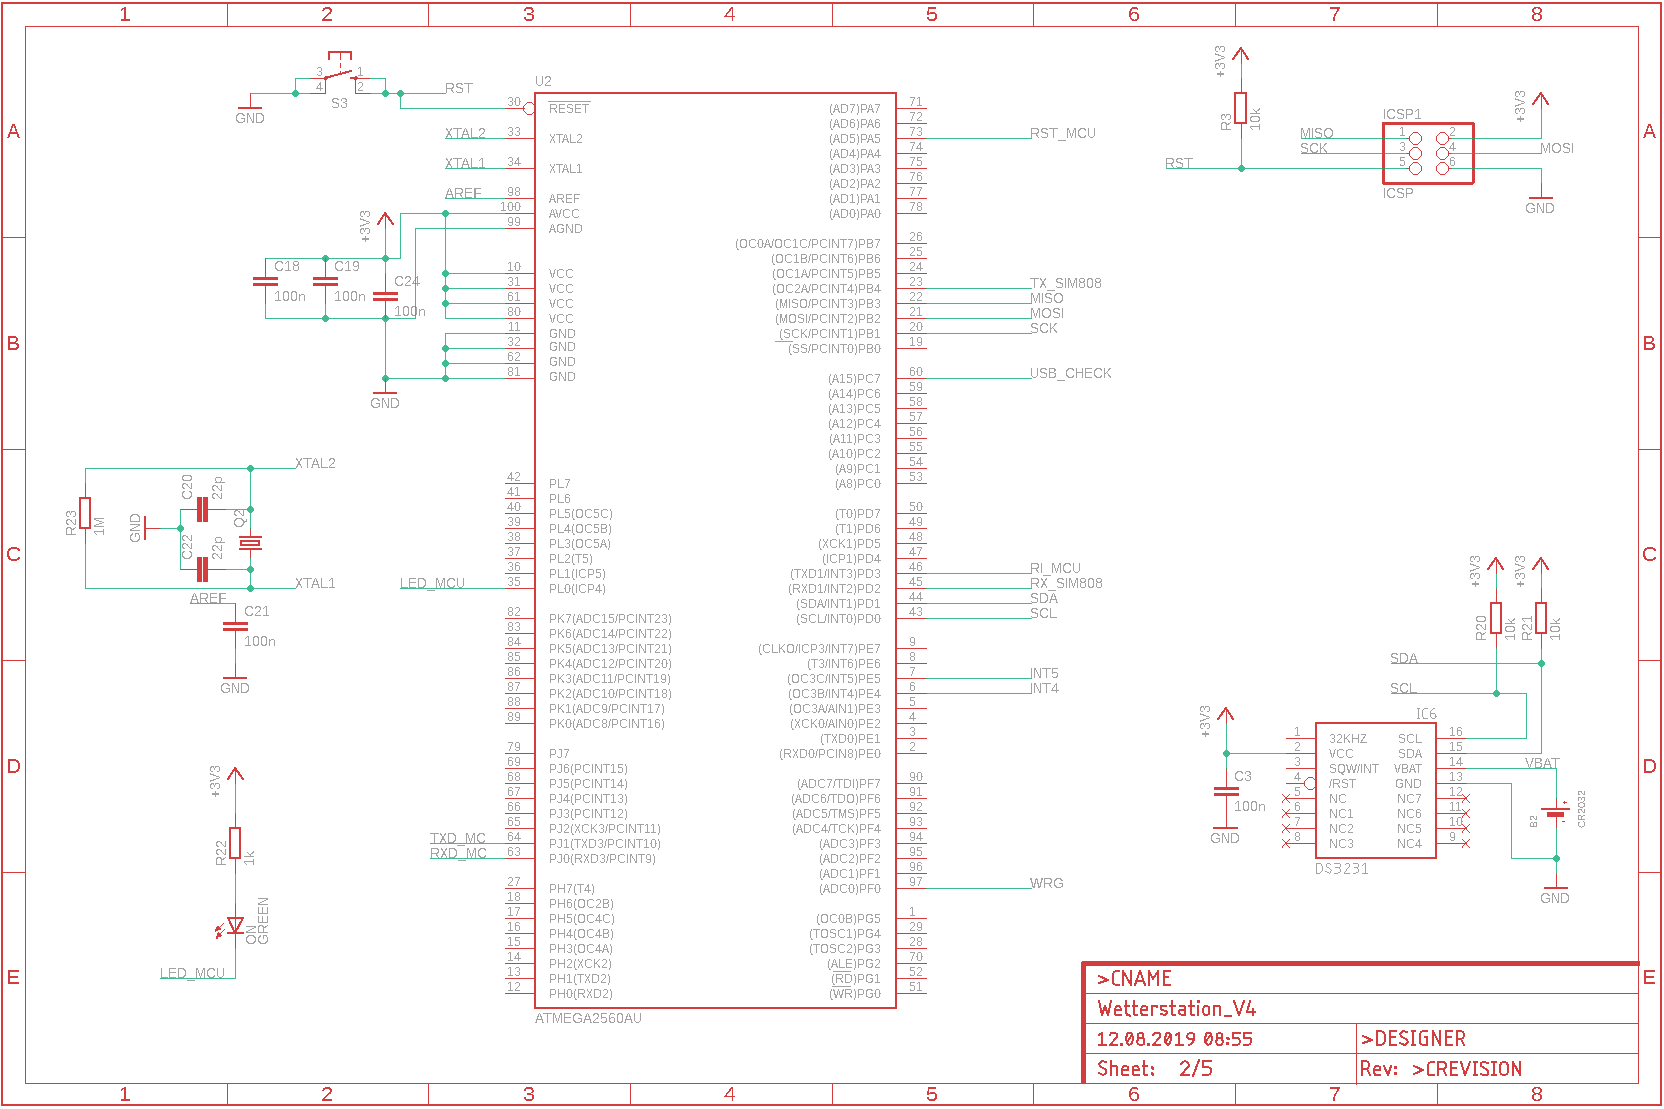
\includegraphics[width=0.7\linewidth]{graphics/Anhang_Eagle/MCU.png}
\caption{Schema der MCU-Bauteilgruppe.}
\label{fig:Anhang_MCU}
\end{figure}
Abbildung \ref{fig:Anhang_MCU} zeigt das Schema der MCU-Bauteilgruppe.
\newpage
\begin{figure}[h]
\centering
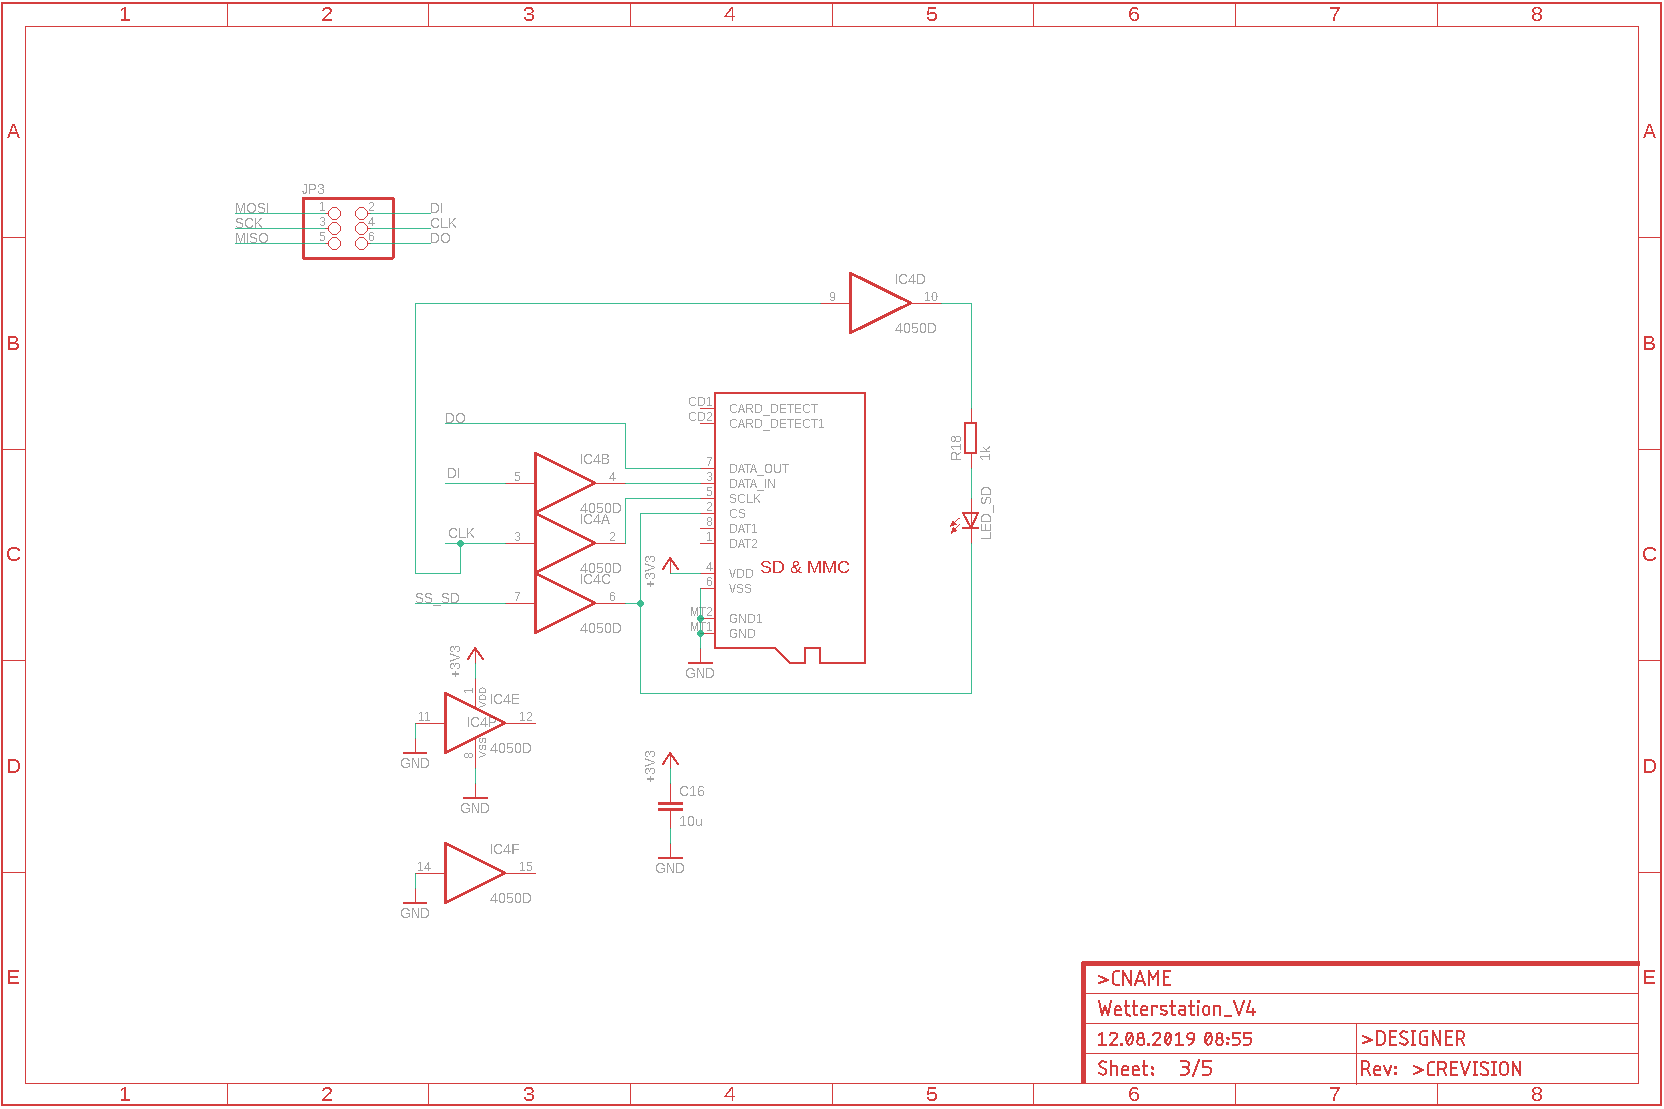
\includegraphics[width=0.7\linewidth]{graphics/Anhang_Eagle/uSDCard.png}
\caption{Schema der $\mu$SD-Bauteilgruppe.}
\label{fig:Anhang_uSDCard}
\end{figure}
Abbildung \ref{fig:Anhang_uSDCard} zeigt das Schema der Datenspeicherungs-Bauteilgruppe.
\newpage
\begin{figure}[h]
\centering
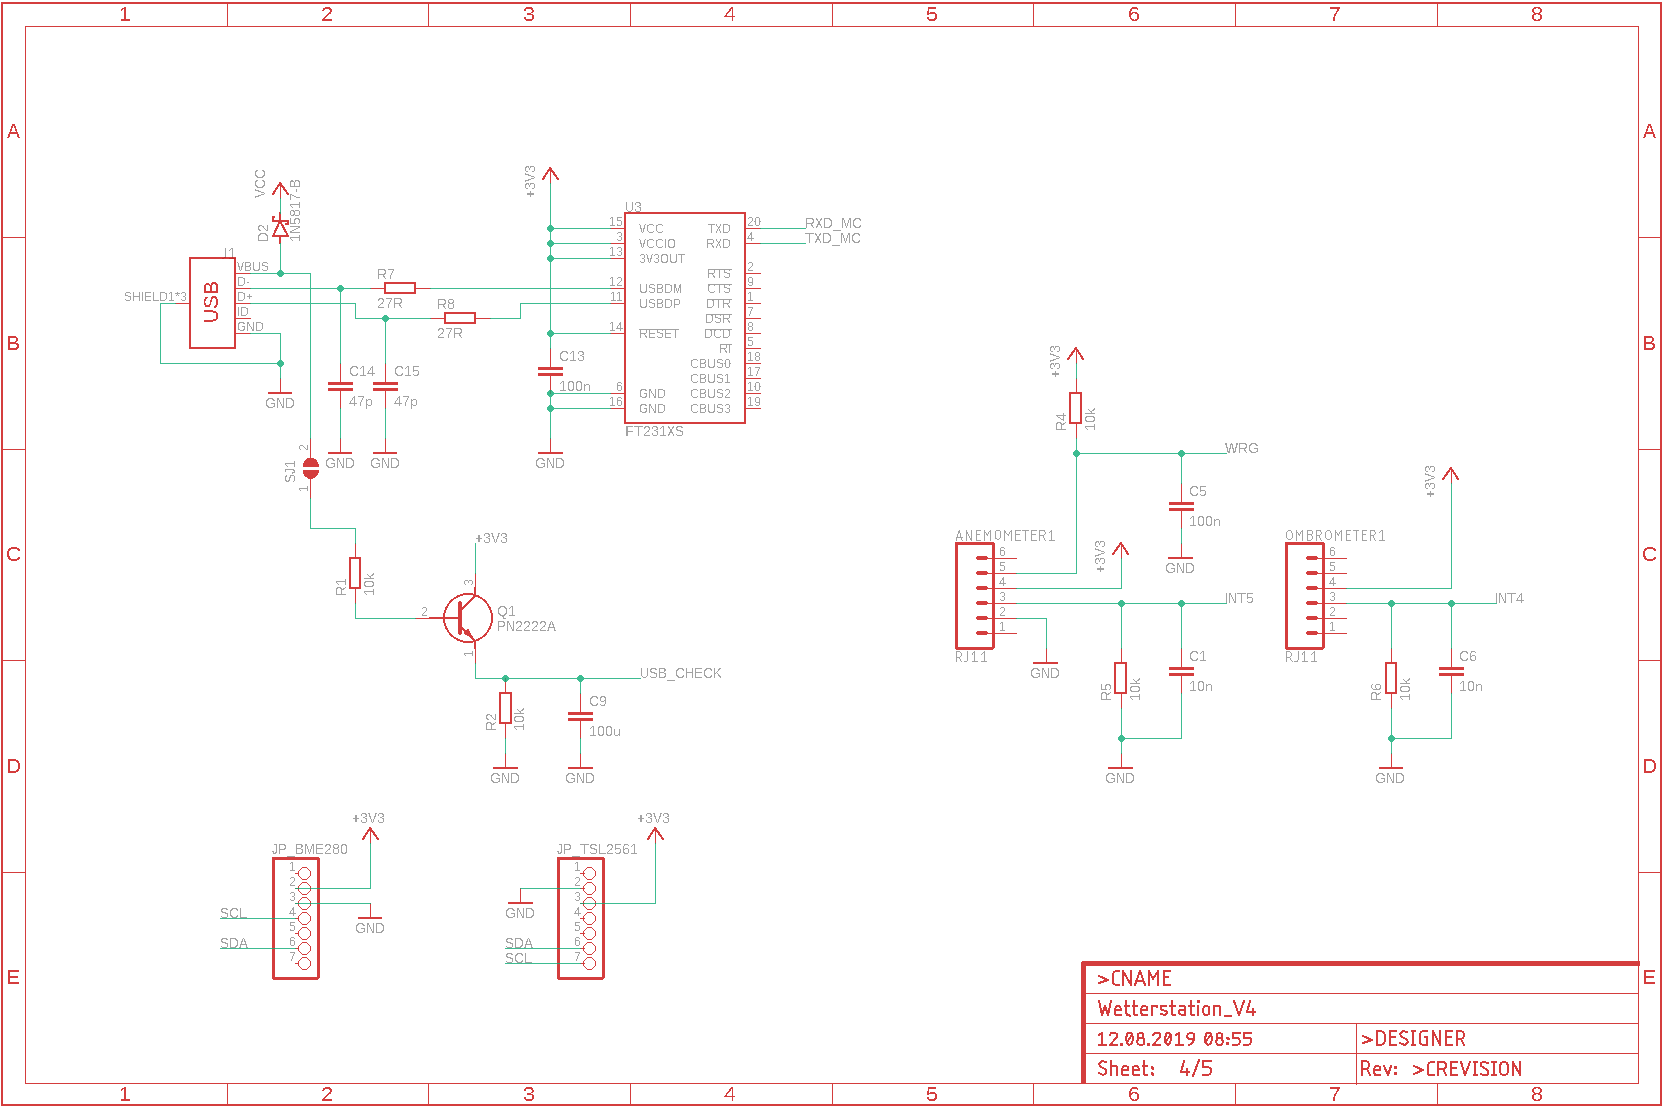
\includegraphics[width=0.7\linewidth]{graphics/Anhang_Eagle/IfAndSense.png}
\caption{Schema des $\mu$USB-Anschlusses und der Sensorik.}
\label{fig:Anhang_IfAndSense}
\end{figure}
Abbildung \ref{fig:Anhang_IfAndSense} zeigt das Schema der seriellen Schnittstelle und der Sensorik.
\newpage
\begin{figure}[h]
\centering
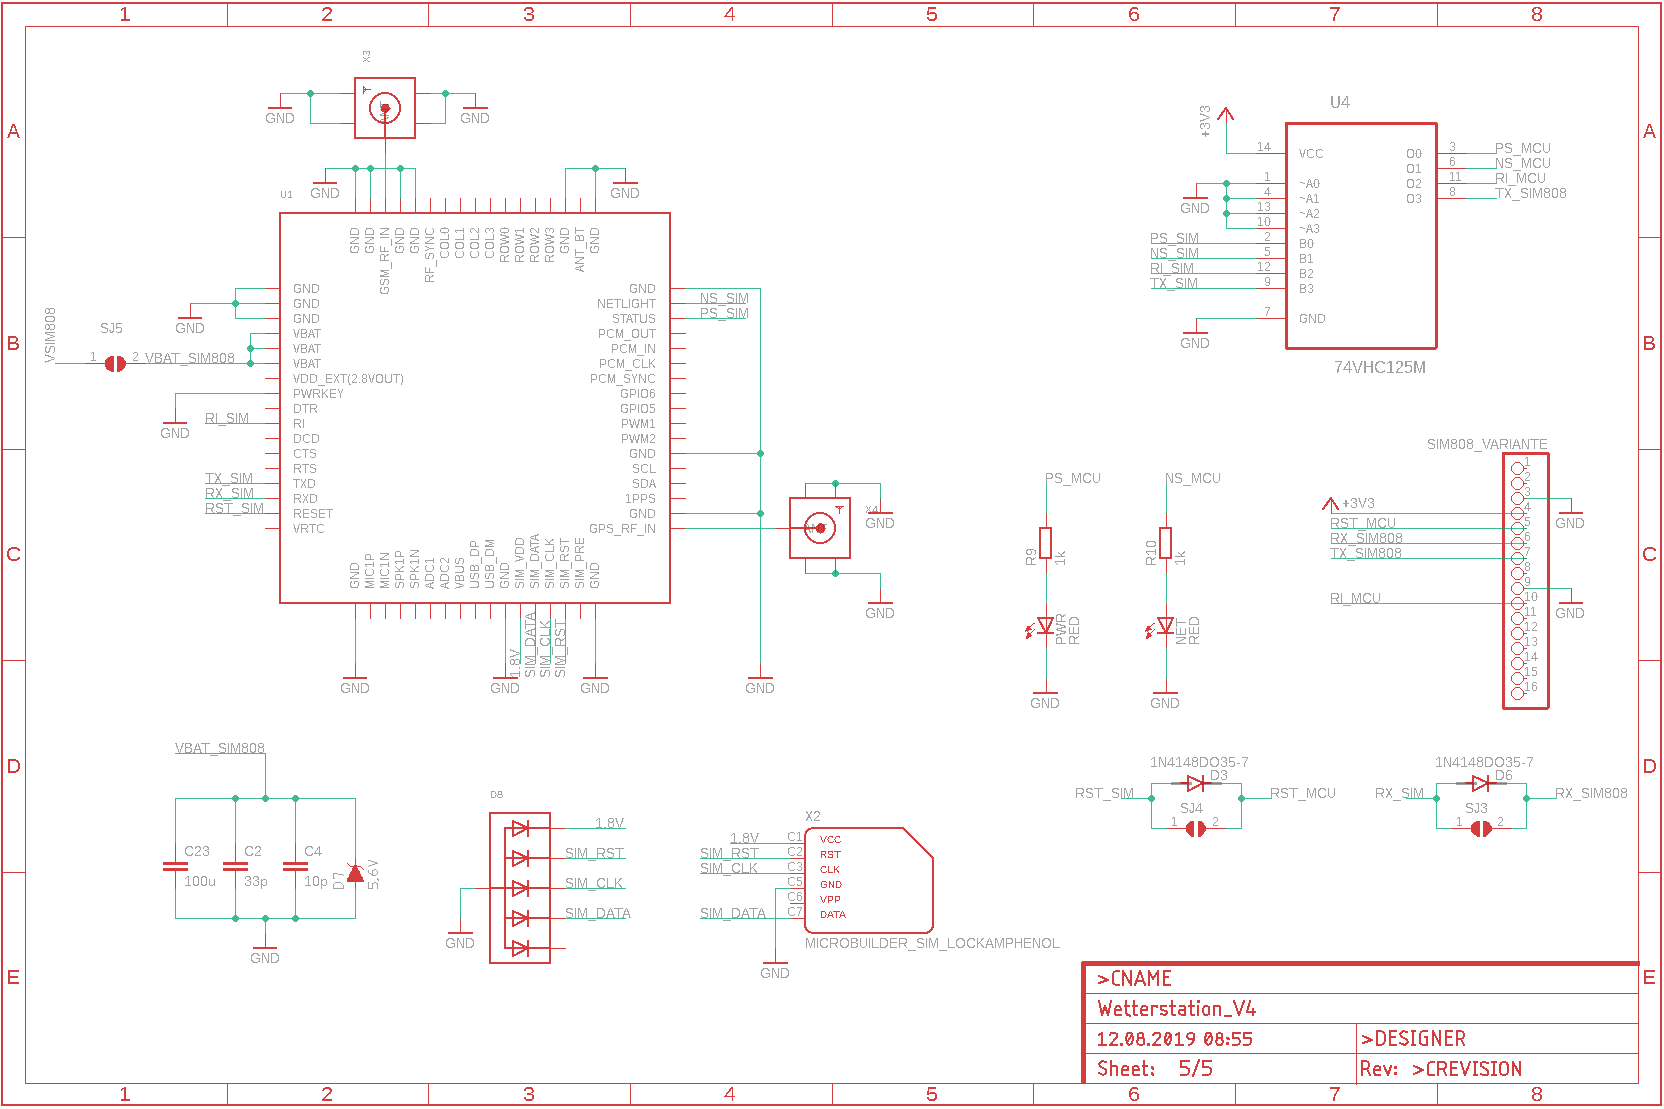
\includegraphics[width=0.7\linewidth]{graphics/Anhang_Eagle/SIM808.png}
\caption{Schema des SIM808.}
\label{fig:Anhang_SIM808}
\end{figure}
\ref{fig:Anhang_SIM808} zeigt das Schema der SIM808-Bauteilgruppe.
\end{landscape}
\newpage
\section{PCB-Layout}
\label{Anhang:PCB}
\begin{figure}[h]
\centering
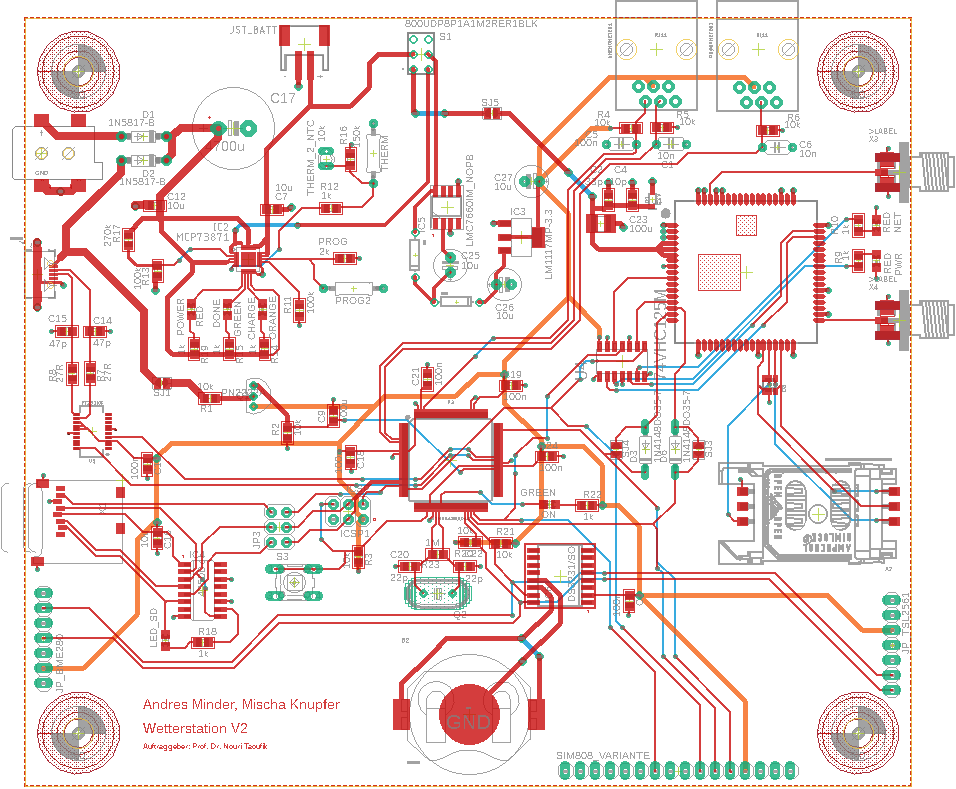
\includegraphics[width=0.99\linewidth]{graphics/Anhang_Eagle/PCB.png}
\caption{Das PCB-Layout der Wetterstation.}
\label{fig:Anhang_PCBLayout}
\end{figure}
Abbildung \ref{fig:Anhang_PCBLayout} zeigt das PCB-Layout der Wetterstation. Es sind deutlich die verwendeten Bauteile zu erkennen, die Bohrlöcher, Vias und verschiedenfarbige Linien. Rote Linien sind auf dem obersten Layer (Layer 1), welcher hauptsächlich für Signale verwendet wird. Der zweitoberste Layer (Layer 2) ist mit einer Groundfläche (0V) ausgefüllt und wird über Vias angesteuert. Der zweitunterste Layer (Layer 3) dient dem 3.3V-Netz um die Bauteilgruppen zu Speisen (Orange). Der unterste Layer (Layer 4) ist ebenfalls für Signale reserviert (Blau), um anderen Leiterbahnen besser Ausweichen zu können. Etwaige Wechsel zwischen Layer 1 und Layer 4 werden mit durchgehenden Vias gemacht. Wechsel zwischen Layer 1 und Layer 2 bzw. Layer 3 werden mit blind Vias gemacht. Die verschiedenen Layer wurden alle mit Groundflächen ausgefüllt, damit die Herstellung des PCBs dem Hersteller vereinfacht wird (weniger ätzen).

\end{appendix}

